\documentclass[11pt, letterpaper]{article}
\usepackage{graphicx}
\usepackage{amsmath}
\setlength{\topmargin}{-2cm}
\setlength{\oddsidemargin}{-0.3cm}
\setlength{\textheight}{24cm}
\setlength{\textwidth}{17cm}
\newtheorem{thm}{Theorem}

\begin{document}

\section{The Cauchy-Riemann Conditions}
A single-valued function $f(z)$ of complex variable $z=x+iy$ is analytic if it has derivatives throughout a region of the
complex plane. Or equivalently, a single-valued $f(z)$ is said to be analytic at $z=z_0$ if it has derivatives at $z_0$ and
all points in some neighborhoods of $z_0$.

If we write $f(z) = u(x,y) + iv(x,y)$, then the {\bf necessary} condition for $f(z)$ to be differentiable at a point is
\begin{equation}
	\frac{\partial u}{\partial x} = \frac{\partial v}{\partial y}\,\,\,\,\,\mbox{and}\,\,\,\,\,
	\frac{\partial v}{\partial x} = -\frac{\partial u}{\partial y},
\end{equation}
which is known as the Cauchy-Riemann conditions. The {\bf sufficient} conditions for the differentiability of $f(z)$ at $z_0$ are
\begin{enumerate}
	\item The Cauchy-Riemann condition holds at $z_0$.
	\item The first partial derivatives of $u(x,y)$ and $v(x,y)$ exists and be continuous at $z_0$.
\end{enumerate}
It can be also shown that $\partial f/\partial z^*=0$ if and only if the Cahchy-Riemann conditions holds. This implies that, loosely
speaking, analytic functions are independent of $z^*$, they are functions of $z$ alone.


\section{Complex Integration}
\begin{thm}
{\bf Cauchy's Theorem}: If a function $f(z)$ is analytic within and on a closed contour $C$, and $f'(z)$ is continuous throughout
this region, then
\begin{equation}
	\oint_C f(z) dz = 0.
\end{equation}
\end{thm}
The theorem can be proved without assuming the continuity of $f'(z)$ because any function which is analytic in a region
necessarily has a continuous derivative (cf. the Cauchy-Riemann conditions). If fact, it can be proved that an analytic
function has derivatives of all orders, and therfore its derivatives are continuous. In this sense, we have:
\begin{thm}
{\bf Cauchy-Goursat Theorem}: If a function $f(z)$ is analytic within and on a closed contour $C$, then
\begin{equation}
	\oint_C f(z) dz = 0.
\end{equation}
\end{thm}

Following the Cauchy-Goursat theorem, one can prove the following result which is extremely useful in all mathematical physics:
\begin{thm}
If $f(z)$ is analytic within and on a closed contour $C$, then for any point $z_0$ interior to $C$,
\begin{equation}
	f(z_0) = \frac{1}{2\pi i}\oint_C \frac{f(z)}{z-z_0}dz. \label{CauchyFormula}
\end{equation}
\end{thm}
The theorem shows the amazingly strong inner structure of analytic functions. It means that if a function is analytic
within and on a contour $C$, its value at every point inside $C$ is determined by its value on the bounding curve $C$.

If we differentiate both sides of Eq.~(\ref{CauchyFormula}) with respect to $z_0$ (since $z_0$ is any point inside $C$,
it can be treated as a variable), one obtains
\begin{equation}
	f'(z_0) = \frac{1}{2\pi i}\oint \frac{f(z)}{(z-z_0)^2}dz.
\end{equation}
In general, we have
\begin{equation}
	f^{(n)}(z_0) = \frac{n!}{2\pi i}\oint \frac{f(z)}{(z-z_0)^{n+1}}dz.
\end{equation}
Thus $f(z)$ have derivatives of all orders inside $C$. The $k$th derivative is continuous within $C$ because the $k+1$
derivative exists.

A function that is analytic in the entire complex plane is called an entire function. Thus:
\begin{thm}
{\bf Liouville's Theorem} If $f(z)$ is entire and $|f(z)|$ is bounded for all values of $z$, then $f(z)$ is a constant.
\end{thm}


\section{The Expansion of an Analytic Function}

An important application of the Cauchy-Goursat theorem concerns about the possibility of expanding an analytic function
in a power series. The results are stated as the following theorem.
\begin{thm}
{\bf Laurent's Theorem} Let $f(z)$ be analytic throughout the closed annular region between the two circles $C_1$ and $C_2$
with common center $z_0$. Then at each point in the annulus
\begin{equation}
	f(z) = \sum_{n=-\infty}^{\infty} A_n(z-z_0)^n,
\end{equation}
with the series converging uniformly in any closed region, $R$, lying wholly within the annulus. Here
\begin{equation}
	A_n = \frac{1}{2\pi i}\oint_C\frac{f(z')}{(z'-z_0)^{n+1}}dz',
\end{equation}
for $n=0$, $\pm 1$, $\pm 2$, $\ldots$, and $C$ is any closed contour in the annulus which encloses $z_0$
\end{thm}
A particularly important consequence of Laurent's theorem arises when the function is analytic and has no singularities within
the inner circle $C_2$. This is summarized as the following theorem
\begin{thm}
{\bf Taylor's Theorem} If $f(z)$ is analytic at all points interior to a circle $C$ centered about $z_0$, then in any closed
region contained wholly inside $C$
\begin{equation}
	f(z) = \sum_{n=0}^{\infty}\frac{1}{n!}f^{(n)}(z_0)(z-z_0)^n,
\end{equation}
and this series converges uniformly.
\end{thm}


\section{Residue Theory}
This is really just an application of the above theorems
\begin{thm}
{\bf The Residue Theorem} The integral of $f(z)$ around a closed contour $C$ containing a finite number $n$ of singular points
of $f(z)$ equals the sum of $n$ integrals of $f(z)$ about $n$ circles, each enclosing one and only one of the $n$ singular
points. In other words,
\begin{equation}
	\oint_C f(z)dz = 2\pi i\sum_{j=1}^n R_j,
\end{equation}
where $R_j$ is called the residue at the point $z_j$:
\begin{equation}
	R_j = \frac{1}{2\pi i}\oint_{C_j}f(z)dz. \label{residue}
\end{equation}
\end{thm}
In addition to the definition Eq.~(\ref{residue}), there is another way of computing residues which is sometimes useful.
If we expand $f(z)$ in a Laurent series about the singular point $z_0$:
\begin{equation}
	f(z) = \sum_{n=0}^\infty a_n(z-z_n)^n + \sum_{n=1}^\infty b_n(z-z_0)^{-n}.
\end{equation}
It can be shown that
\begin{equation}
	b_1 = \frac{1}{2\pi i}\oint_{C_0}f(z)dz \equiv R_0.
\end{equation}
In other words, the residue around a point $z_0$ can be found by expanding the function around $z_0$ in a Laurent
series and picking out the coefficient of the term in $(z-z_0)^{-1}$.


\section{Evaluation of definite integrals}

\subsection{$\displaystyle\int_0^{2\pi}R(\cos\theta, \sin\theta)d\theta$}
\label{sec:a}
Here $R(\cos\theta, \sin\theta)$ is a rational function
\begin{equation}
	R(\cos\theta, \sin\theta) = \frac{a_1\cos\theta + a_2\sin\theta + a_3\cos^2\theta + \ldots}
									 {b_1\cos\theta + b_s\sin\theta + b_3\cos^2\theta + b_4\sin^2\theta + \ldots}
\end{equation}
To evaluate the integral, we let $z=e^{i\theta}$ and proceed with the substitution
\begin{equation}
	\cos\theta = \frac{1}{2}\left(z + \frac{1}{z}\right),\,\,\,\,\,\,
	\sin\theta = \frac{1}{2}\left(z - \frac{1}{z}\right),
\end{equation}
and $d\theta = -i(dz/z)$. The integral becomes
\begin{equation}
	-i\oint_C R\left[\frac{1}{2}\left(z + \frac{1}{z}\right), \frac{1}{2}\left(z - \frac{1}{z}\right)\right]\frac{dz}{z},
\end{equation}
where $C$ is the unit circle.


\subsection{$\displaystyle\int_{-\infty}^{\infty}R(x)dx$}
\label{sec:b}
In this case, $R(x)$ is a rational function without poles on the real axis. Furthermore, suppose the degree of the
denominator of $R(x)$ is at least two unit higher than the degree of the numerator, meaning $|R(z)|\rightarrow 1/|z^2|$
as $|z|\rightarrow\infty$, and all the singularities of $R(z)$ are in the upper half-plane, then 
\begin{equation}
	\int_{-\infty}^\infty R(x)dx = \oint_C R(z)dz = 2\pi i\sum_{y > 0} \mbox{Res}\,R(z).
\end{equation}
where $C$ encloses all singularities in the upper half-plane.

\begin{figure}
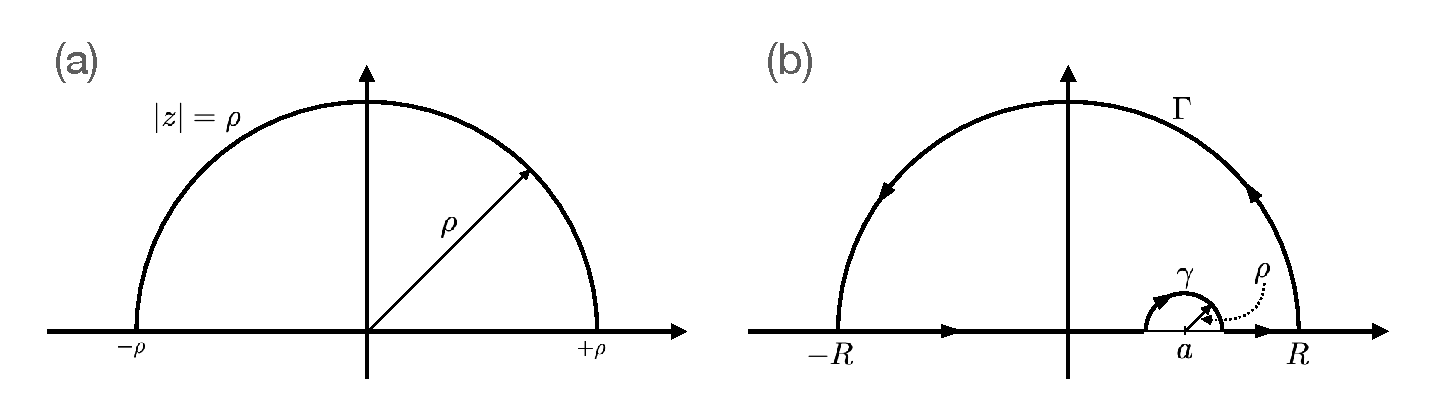
\includegraphics[width=\textwidth]{./figures/fig_complex_analysis.pdf}
\caption{(a) Contour for the integrals considered in \ref{sec:d}. (b) Contour for the integrals considered in \ref{sec:e}}
\label{fig:contour}
\end{figure}

\subsection{$\displaystyle\int_{-\infty}^{\infty}R(x)e^{ix}dx$}
\label{sec:c}
Again, assuming there are no poles on the real axis, and if the raional function $R(z)$ has a zero of at least order two
at infinity, then
\begin{equation}
	\int_{-\infty}^{\infty}R(x)e^{ix}dx = \oint_C R(z)e^{iz}dz = 2\pi i\sum_{y>0}\mbox{Res}\,\left[R(z)e^{iz}\right]
\end{equation}

\subsection{$\displaystyle\int_{-\infty}^{\infty}R(x)e^{i\alpha x}dx$}
\label{sec:d}
Here $R(x)$ has a zero of order one at infinity, and again, it is assumed that there are no poles on the real axis.
To evaluate the integral, we consider a contour consisting of a semi-circle in the upper half-plane and the real axis
and write:
\begin{equation}
	\oint_C R(z) e^{i\alpha z}dz = \lim_{\rho\rightarrow\infty}\int_{-\rho}^\rho R(x)e^{i\alpha x}dx +
								   \int_{semi, |z|=\rho}R(z)e^{i\alpha z}dz.
\end{equation}
For $\alpha > 0$, the Jordan's Lemma tells us that the integral over the semi-circle vanishes. The integral on the
left hand side is given by the residue theory. Thus
\begin{equation}
	\int_{-\infty}^{\infty}R(x)e^{i\alpha x}dx = 2\pi i\sum_{y>0}\mbox{Res}\,\left[ R(z)e^{i\alpha z}\right]
\end{equation}


\subsection{$\displaystyle\int_{-\infty}^{\infty}Q(x)dx$}
\label{sec:e}
We consider the function $Q(z)$ and assume that it is meromorphic (i.e. no essential singularities) in the upper half-plane,
and has poles of order one (i.e. simple poles) on the real axis. If $Q(z)$ behaves at infinity like any of the integrands
discussed in \ref{sec:b}, \ref{sec:c}, or \ref{sec:d}, then we can extend those techniques and, using the contour shown
in Fig.~\ref{fig:contour}(b), evaluate the integral as follows
\begin{equation}
P\int_{-\infty}^{\infty}Q(x)dx = 2\pi i\sum_{y>0}\mbox{Res}\,Q(z) + \pi i\sum_{y=0}\mbox{Res}\,Q(z),
\end{equation}
where the second term denotes the sum of the residues of $Q(z)$ at each of its simple poles on the real axis.


\begin{figure}
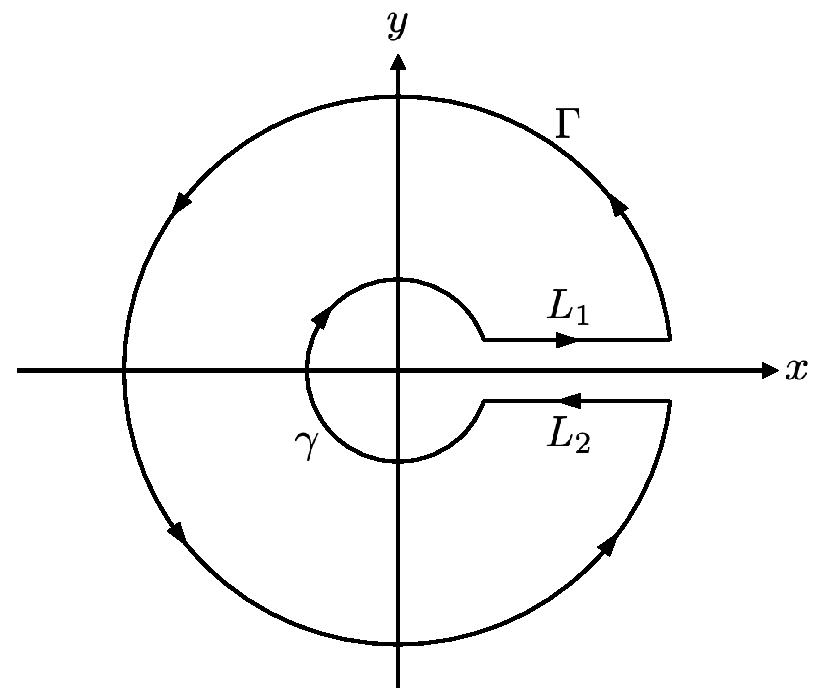
\includegraphics[width=0.45\textwidth]{./figures/fig_complex_analysis2.pdf}
\caption{Contour for the integrals considered in \ref{sec:f}.}
\label{fig:contour2}
\end{figure}

\subsection{$\displaystyle\int_0^{\infty} x^{\lambda-1}R(x)dx$}
\label{sec:f}
In this last case, we assume that $\lambda$ is not an integer. $R(z)$ is rational and analytic at $z=0$, and has no poles on the
positive real axis, and $|z^\lambda R(z)|\rightarrow 0$ uniformly as $|z|\rightarrow 0$ , and as $|z|\rightarrow \infty$.
This problem invloces branch points and branch cuts because the power function $z^{\lambda-1}$ is in general not a single-valued
function. In the current case,  $z^{\lambda-1}$ has a branch point at the origin. We can consider the following branch of the
function ($z=re^{i\theta}$)
\begin{equation}
	z^{\lambda-1} = \exp\left[(\lambda-1)\log z\right] = \exp\left[(\lambda -1)(\log r+ i\theta)\right],
\end{equation}
where $0 < \theta < 2\pi$ and $r > 0$. 

Now consider the contour shown in Fig.~\ref{fig:contour2}. Because of the branch cut along the positive real axis:
\begin{equation}
	\oint z^{\lambda-1}R(z)dz = \int_\Gamma + \int_\gamma + \int_{L_1} + \int_{L_2}.
\end{equation}
Since the cut is along the positve real axis, the line integrals above and below the cut will not cancel. In fact, 
along the line $L_1$, we have $z=x$, the usual convention. For the line just below the cut, $z = x e^{2\pi i}$
since it picks up a $2\pi$ phase. The integrals over $\Gamma$ and $\gamma$ vanish, because
$|z^\lambda R(z)|\rightarrow 0$ as $|z|\rightarrow 0$, and as $|z|\rightarrow \infty$. Thus
\begin{align}
	\oint z^{\lambda-1}R(z)dz 
		&= \int_\infty^0 e^{2\pi i (\lambda-1)}x^{\lambda-1}R(x)dx + \int_0^\infty x^{\lambda-1}R(x)dx. \nonumber\\
		&= \frac{-2i\sin\pi\lambda}{e^{-\pi i\lambda}}\int_0^\infty x^{\lambda-1}R(x)dx
\end{align}
The left hand side of the above equation is nothing but the sum of residues inside the contour:
\begin{equation}
	\oint z^{\lambda-1} R(z)dz = 2\pi i\sum_{interior} \mbox{Res}\,\left[z^{\lambda-1}R(z)\right]
\end{equation}
Thus it follows that
\begin{equation}
	\int_0^\infty x^{\lambda-1}R(x)dx = \frac{\pi(-1)^{\lambda-1}}{\sin\pi\lambda}
				\sum_{interior} \mbox{Res}\,\left[z^{\lambda-1}R(z)\right].
\end{equation}

\begin{thm}
Let $f(z)$ be a meromorphic function (i.e. no essential singularities) and let $C$ be a contour which encloses
the zeros of $\sin\pi z$, located at $z=\rho$, $\rho+1$, $\ldots$, $n$. If we assume the poles of $f(z)$ and
$\sin\pi z$ are distinct, then
\begin{equation}
	\sum_{m=\rho}^n f(m) = \frac{1}{2\pi i}\oint_C \pi\cot\pi z\,f(z)dz 
			- \sum\mbox{Res}\,\left[\pi\cot(\pi z)\,f(z)\right]
\end{equation}
where the summation on the right hand side is over poles of $f(z)$ inside $C$.
\end{thm}


\section{Reference}
\begin{enumerate}
	\item Mathematics of Classical and Quantum Physics, Frederick W. Byron Jr. and Robert W. Fuller.
\end{enumerate}
\end{document}